\documentclass[10pt,a4paper,onecolumn,titlepage]{article}
\usepackage[utf8]{inputenc}
\usepackage[croatian]{babel}
\usepackage{amsmath}
\usepackage{amsfonts}
\usepackage{amssymb}
\usepackage{graphicx}

\title{Višekorisnička chat aplikacija u C\#-u}
\author{Antonio Kovačić\\Janko Marohnić\\Lana Arzon}

\begin{document}
\maketitle

\tableofcontents

\newpage

\section{Opis problema}

Potrebno je napraviti aplikaciju za gdje se ljudi mogu međusobno dopisivati
u realnom vremenu. Dvije ili više osoba se treba moći "naći na jednom mjestu",
i komunicirati zajedno putem tekstualnih poruka.

Kada se osoba prijavi u chat, treba upisati svoje korisničko ime, kojim će se
ta osoba identificirati. Ako je postoji druga osoba u istoj "sobi" koja već
ima željeno korisničko ime, osoba bi trebala izabrati drugo korisničko ime.
Nakon što je upisala korisničko ime, osoba mora moći vidjeti koji su sve drugi
korisnici trenutno prijavljeni u istu "sobu".

Kada osoba pošalje poruku u grupni chat (napiše teskt i stisne "enter"), svaka
druga osoba mora primiti tu istu poruku (i treba pisati od koga dolazi). Na taj
način svatko zna što su svi ostali rekli. I poruke moraju stizati redom kojim
su poslane.

Kada se osoba odjavi iz chata, ostalim osobama treba doći poruka da se ta
osoba odjavila iz chata.

\section{Implementacija}

\subsection{Server}

\subsubsection{Kreiranje}

\subsubsection{Instaliranje}

\subsubsection{Pokretanje}

\begin{figure}[!ht]
\begin{minipage}{\textwidth}
\centering
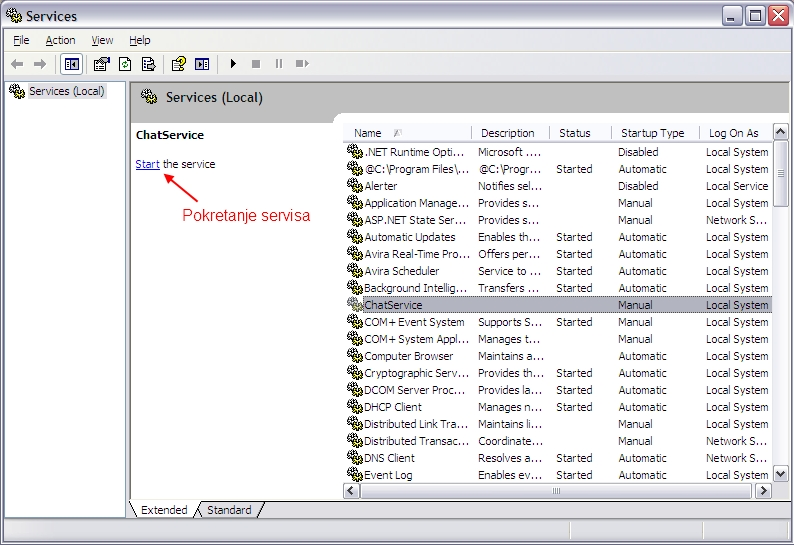
\includegraphics[width=\textwidth]{images/start_service.jpg}
\caption{Pokretanje servisa ChatService}
\end{minipage}
\end{figure}

\subsection{Klijent}

...

\end{document}
